\documentclass[../../../Aurora C# unofficial manual.tex]{subfiles}

\begin{document}
	\section{Unit design}
	Original post can be found
	\href{http://aurora2.pentarch.org/index.php?topic=8495.msg105824#msg105824}{here}.
	\\\\
	
	Ground Forces and Ground Combat are undergoing a huge expansion in C\#. The VB6 Ground Unit becomes the Formation and the VB6 Ground Unit Type becomes the Formation Template. However, there are no longer any fixed unit types or unit values. Instead, there is endless scope for Formations and Formation Templates, based on a detailed design process at the Formation level and below. This will allow the simulation of ground forces from many science fiction genres. As this is a long topic, I am going to break it into several posts each covering a different topic.
	
	The most granular level is the Ground Unit Class, which is an individual soldier or vehicle. One or more of the same Ground Unit Class are grouped into Formation Elements, which in turn are grouped into Formations. Formations remain intact for movement purposes, but combat involves each individual unit (each soldier or vehicle). As individual units are now tracked for casualty purposes, readiness no longer exists. Morale is tracked at the Formation Element level (which is a group of the same unit class), so the infantry in a Formation may have a different morale than the anti-tank guns or artillery.
	
	The process of design starts with the Ground Unit Class. Two important factors in this design process are the Racial Armour Strength and Racial Weapon Strength, shown at the top of the Ground Forces window.
	
	Racial Armour Strength is based on the strength of the highest racial armour technology. Conventional Armour is 3, Duranium Armour is 5, et cetera. For this screenshot, the Commonwealth has researched Ceramic Composite, which has a strength of 10.
	
	Racial Weapon Strength is based on the highest tech level (TL) among Laser Focal Size, Railgun Type, Meson Focal Size, Particle Beam Strength and Carronade Calibre. For example, 15cm Laser Focal Size is TL3 as it is the third tech of that type. Racial Weapon Strength is the value of armour at the same tech level. In this case, the Commonwealth has researched 20cm Laser Focal Size, which is TL4. The fourth Armour Tech is Ceramic Composite, which has a strength of 10, so the Racial Weapon Strength is 10. The reason for using Armour as the basis of Weapon Strength is partly because that means Ground Armour and Ground Weaponry are aligned, and partly because it is straightforward way to assign value based on very different weapons.
	
	The Ground Unit Design tab of the new ground Forces window is shown below. First, a 'base type' is chosen, which is infantry, several sizes of vehicle, or static. Static in this sense is a weapon that is not self-mobile, such as a towed anti-tank gun, towed artillery, et cetera. Static weapons remain in place when firing so they are easier to hit than infantry or vehicles. Each base type has six main characteristics:
	\begin{enumerate}
		\item Size (in tons): Size is the basis for transport requirements and cost, although there are other modifiers to cost (discussed below).
		\item Hit Points: Unit hit points are compared to weapon damage during combat to determine the chance of destruction (the Damage Check). The chance of a weapon destroying a unit is \( (Weapon Damage / Hit Points)^{2} \).
		\item Slots: The number of component slots available for the base type.
		\item To-Hit Modifier: Used to modify the chance of the unit being hit during combat (based on the mobility of the unit). This only applies if the unit is not fortified.
		\item Maximum Fortification: The maximum strength to which the unit can be fortified by construction factories or construction units. The Chance to Hit for a firing unit is divided by the Fortification Level of the target unit.
		\item Maximum Self-Fortification: The maximum strength to which the unit can be fortified without construction factories or construction units.
	\end{enumerate}
	
	The next section is Armour Type. The Armour of a unit is compared to the Armour-Penetration (AP) value of a weapon. The chance to penetrate is equal to \( (AP / Armour)^{2} \). For example, a weapon with AP 4 attacking a unit with Armour 6 has a 45\% chance to penetrate. The overall process for checking if a shot destroys a target is Chance To-Hit, followed by Armour Penetration Check, followed by Damage Check. All three must be successful to destroy the target. Each type of Armour has two values.
	\begin{enumerate}
		\item Base AR: The Base Armour Rating is multiplied by Unit Size (including components below) to determine cost. So a unit with 6 armour would be 50\% more expensive than the same unit with 4 armour.
		\item Racial AR: Racial Armour Rating is the Base Armour Rating multiplied by the Racial Armour Strength (shown at top of window).
	\end{enumerate}
	
	Below the base type and armour is a large section showing Components. Infantry, static and light vehicles all have one 'component slot', vehicles and heavy vehicles have two slots, while super-heavy and ultra-heavy vehicles have three and four slots respectively. Each slot can hold one component from the list and the same component can be put into multiple slots. Certain components are only available with certain base types. For example, the Super-Heavy Anti-Vehicle component can only be used by super-heavy and ultra-heavy vehicles. The primary component is selected from the main table, while any additional components are selected from the dropdown(s) below the main table. Each component has a name and an abbreviation and is rated in nine different areas:
	\begin{enumerate}
		\item Size: The size in tons is added to the size of the base unit type.
		\item Armour-Penetration (AP): If the component is a weapon, the chance to penetrate a target's armour is \( (AP / Armour)^{2} \). The AP Rating is the underlying AP of the component (not shown), multiplied by the Racial Weapon Strength.
		\item Damage:  If the component is a weapon, the chance to destroy a target after the armour has been penetrated is \( (Weapon Damage / Hit Points)^{2} \). The damage value is the underlying damage rating of the component (not shown), multiplied by the Racial Weapon Strength.
		\item Shots: The number of times a weapon will fire during each ground combat phase.
		\item CIWS: 'Y' indicates this component is a Close-in-Weapon-System, capable of defending the planet (on which the unit is based) from missile attack. This CIWS will use the values in the CIWS section, which will become visible when a CIWS component is selected. More on this in a later rules post.
		\item STO: 'Y' indicates this component is a Surface-To-Orbit energy weapon, capable of engaging ships in space within weapon range of the planet on which the unit is based. The weapon type used for the STO component can be selected in the section to the centre right, which will become visible when an STO component is selected. More on this in a later rules post, although see the second screenshot.
		\item HQ: The headquarters capacity of the component in tons. This is the total size of the formation (or formation hierarchy) that can be effectively controlled by a commander based in a unit with this component. To assign a commander to a formation, one of the units within that formation requires a headquarters component. More details on command hierarchies will be provided in a future rules post.
		\item FFD: 'Y' indicates this component is a Forward Fire Direction (FFD) component. Forward Fire Direction allows a front-line unit (more on that later) to direct the fire of bombardment units from a formation in a support position, fighters on close air support missions, or ships in orbit. A later rules post will explain this function.
		\item Const. The construction value of the component in Construction Factory Equivalents (CFEs).
	\end{enumerate}
	
	At the top-right of the window is the Capability section. One or more Capabilities can be selected for the Unit Class. The Boarding Combat capability is required for a Unit to be able to board another ship. For all other capabilities, the Chance to Hit is doubled in the environment specified. If a unit has multiple capabilities, such as Mountain Warfare and Jungle Warfare on a world with a dominant terrain of Jungle Mountain, the bonus is cumulative (i.e. 4x to-hit in this case). Each capability selected for a Unit will increase the cost by the multiple specified. Some capabilities are only available for infantry units.
	
	In the bottom right section, a summary of the unit is shown in a similar style to the Class Summary for naval designs. When the sizes of all the units in a formation are aggregated, that is the transport requirement for that formation in tons. Cost is in BP. When the costs of all the units in a formation are aggregated, that is the build point requirement to construct the formation. Armour and Hit Points have been described previously. Below that is a list of components, followed by the materials required for construction and the research cost to develop the unit once designed.
	\begin{figure}[H]
		\centering
		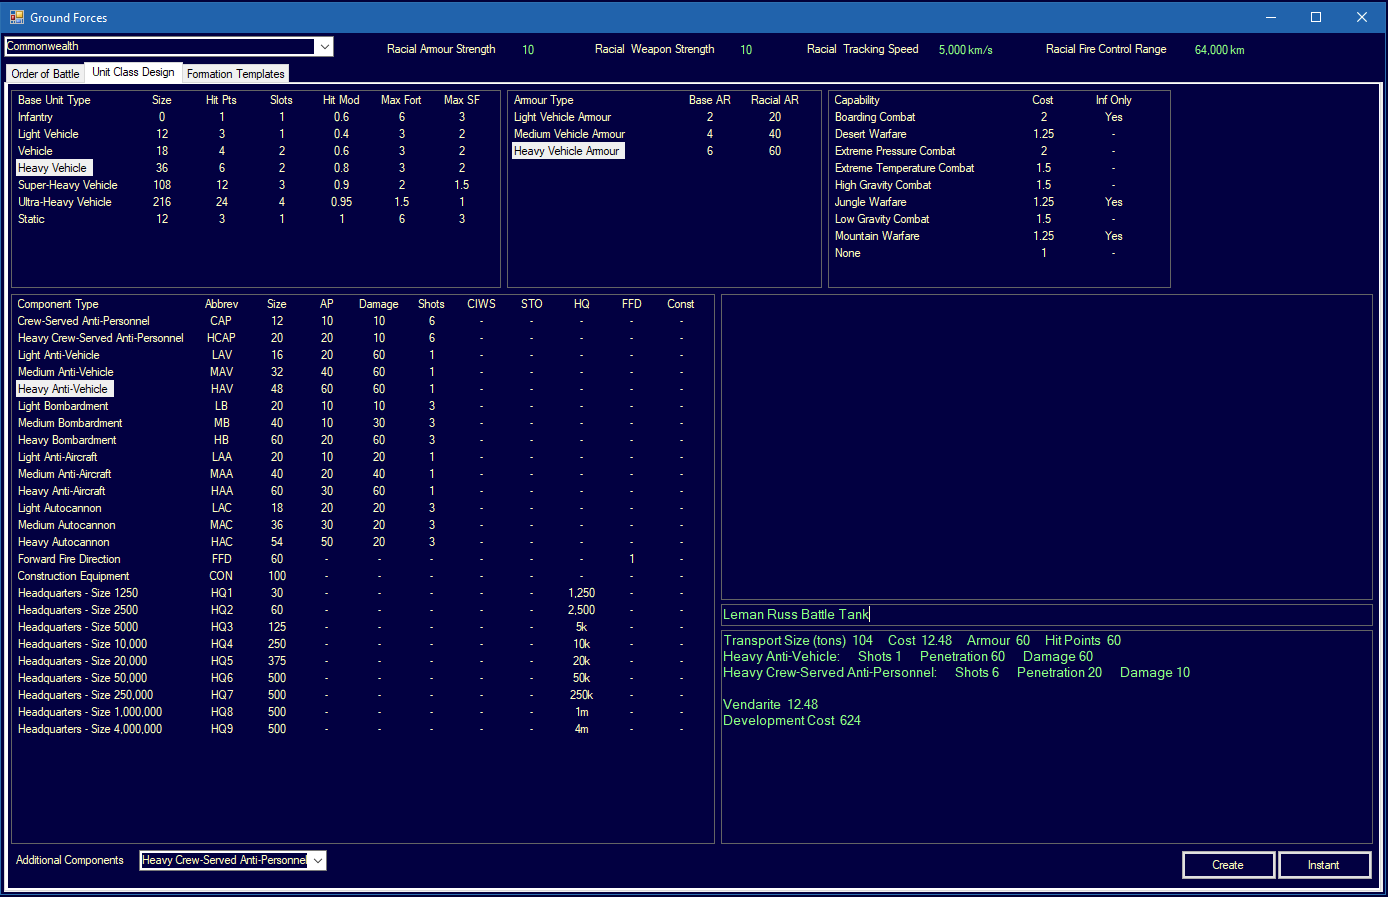
\includegraphics[width=0.9\linewidth]{images/GroundForces}
		\caption[Ground Forces]{Ground Forces Example 1}
		\label{fig:groundforces}
	\end{figure}
	
	This screenshot shows a static unit with an STO component selected. The chosen weapon (which is any non-turreted weapon developed for shipboard use) is selected on the right. Spinal Weapons can be selected for ground use without penalty. The STO mount includes the weapon, a reactor of the exact size needed for the recharge rate, an active sensor with range greater than the weapon range and a built-in beam fire control with a 4x range modifier. The cost is equal to the static platform, the weapon, the reactor, the active sensor and half the fire control. STO weapons have a 25\% bonus to fire control range. The damage shows two numbers, which is the damage at minimum and maximum range.
	\begin{figure}[H]
		\centering
		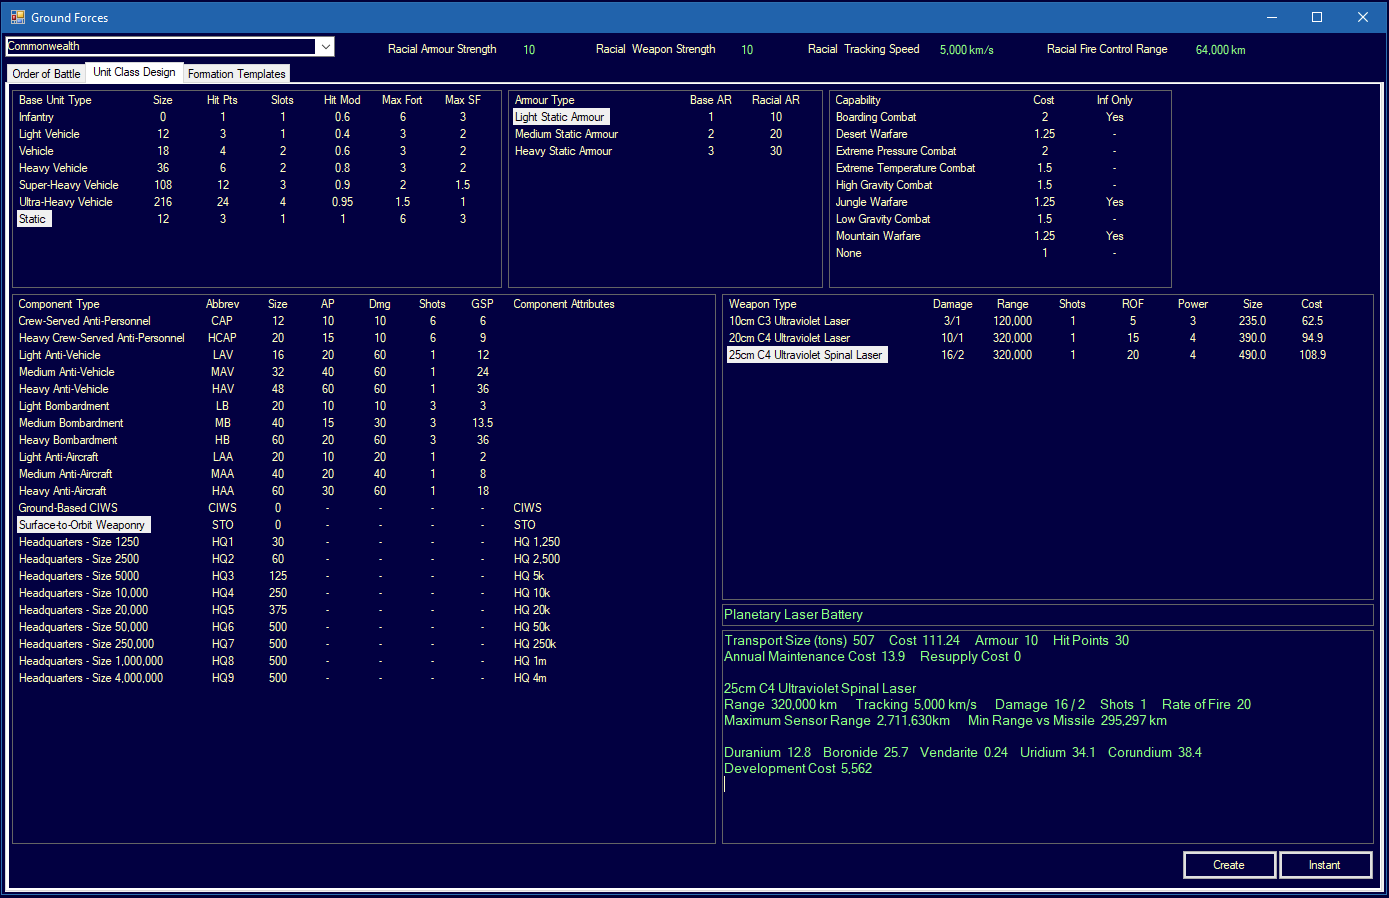
\includegraphics[width=0.9\linewidth]{images/GroundForces2}
		\caption[Ground Forces 2]{Ground Forces Example 2}
		\label{fig:groundforces2}
	\end{figure}
\end{document}